\documentclass[12pt]{scrartcl}
\usepackage{blubird}
% has options [nodate, nosans, nofancy, nocolor, code]

% box setup - should be moved to somewhere nicer
\mdfsetup{
	roundcorner = 2pt,
	linewidth = 1pt,
	innertopmargin = 0.5em,
	innerbottommargin = 1em,
	frametitlefont = \bfseries,
}

% TITLE 
\title{Complex Analysis Notes}
\author{Bryan Lu}
\date{December 2021 - January 2022} % do not use if [nodate] option enabled
 
\begin{document}
\maketitle

\setcounter{section}{-1}
\section{Foreword}
These are notes for the FA21 MATH 2230 study group for complex analysis over break. These are intended as a summary of the material presented in Stein-Shakarchi and Ahlfors, with supplements from Chapter V of \textit{Advanced Mathematical Techniques for Scientists and Engineers} by Osborne.

Complex analysis is a wonderful subfield of analysis and is useful for a lot of math/physics majors! It's relatively independent from the study of real analysis, and arguably (in my opinion) it's a lot more fun and elegant than its real counterpart! :)

Some prerequisites -- if you've taken MATH 2230 at Cornell, this should be accessible to you. Otherwise, the prerequisites are an interest in rigor, and some level of mathematical sophistication, i.e. some exposure to real analysis, particularly in regards to limits, continuity, and differentiation, and of course at least some familiarity with manipulating complex numbers. Some basic notions will be skimmed over here, as... well... it's really very similar to analysis in $\RR^2$ in this respect so we skim over it with the intention of  focusing on the highlights instead.

Many of the earlier diagrams in these notes are courtesy of Mathematica -- it can make some pretty cool stuff! Unfortunately, as of the time of writing I temporarily cannot generate these plots. :( Later diagrams that are not computer generated are drawn in Inkscape and hopefully look pretty clean.

\pagebreak

\section{Welcome to Complex Land!}
Analysis, of course, is a rigorous discipline that gives us a lot of the structure underlying calculus. However, the point of this first section is to be less concerned with the rigor and is more focused on introducing ourselves to some of the common actors.

\subsection{The Stage: The Complex Numbers}
Welcome to $\CC$, the set of numbers over which we will assume to be working with in the entirety of these notes! We will take the following as our definition of $\CC$:
\[
    \CC = \{ a + b i : a, b, \in \RR, i^2 = -1\}
\]
This will serves our purposes just fine. $\RR$, of course, is the normal field of real numbers, which I hope we're all familiar with. If we were super concerned about rigor, this loose definition can be made into a more rigorous construction of $\CC$, but we'll refrain from doing so here.

We will endow the complex numbers with the standard operations of a field (addition and multiplication), and we'll assume you know how these operations work already, but just for the sake of defining it:
\[(a + bi) + (c + di) = (a + c) + (b+ d) i.\]
\[(a + bi) \cdot (c + di) = (ac - bd) + (ad + bd)i. \]
Every complex number $z = a + bi$ also has a \textit{conjugate}, $\bar z = a - bi$.

I would like to focus more on endowing the complex numbers with a geometric interpretation as being similar to $\RR^2$ by plotting them on the plane, like so:
%% diagram - complex plane w/ arbitrary complex number, stuff labeled
In this case, we see that we can also represent any complex number $z$ in a polar form -- in particular, in terms of its distance to the origin, and the angle it makes with the positive real axis. We can thus write
\[
    z = r (\cos \theta + i \sin \theta),
\]
where $r$ is a non-negative real number, and $\theta$ is any real number. We call $r$ the \textit{modulus} (or magnitude, or norm) of $z$, $|z|$, and $\theta$ the \textit{argument} of $z$, $\arg z$.

Before discussing the argument further, we first establish \textit{Euler's Formula} (one of them) which establishes that
\[
    e^{i\theta} = \cos \theta + i \sin \theta = \cis \theta.
\]
I personally strongly favor the exponential form over the cis form, unless I can't avoid it.

There are many ways to show that this is true depending on what initial conditions one has -- we could do this by simply employing a Taylor series expansion and comparing terms. Another way that might be more convincing if we don't believe we should be using Taylor over the complex field is through a differential equations approach. Note that
\[
    \dv{}{\theta} \cis \theta = -\sin \theta + i \cos \theta = i(i \sin \theta + \cos \theta) = i \cis \theta
\]
Now, for the definition of $e^z$ such that $e^z$ is the unique solution to the initial value problem $y' = y$, $y(0) = 1$, we can infer from the chain rule that $e^{iz}$ satisfies this equation, proving the statement.

Geometrically, this statement allows us to think of complex number multiplication in a nice way, if we choose to work in polar coordinates. If for two complex numbers $z$ and $w$ we have $z = r_1 e^{i\theta_1}$ and $w = r_2 e^{i\theta_2}$, we have that $zw = r_1 r_2 e^{i (\theta_1 + \theta_2)}$, i.e. the argument adds and the magnitudes multiply, by nature of the exponential properties.

Okay, but back to the argument. The argument of $z$ is not a function, because of the periodicity in $\sin$ and $\cos$: $\cis 2\pi = e^{2i \pi} = 1$, so that means that if $z = re^{i\theta}$, $z$ is also $re^{i(\theta + 2pi)}$. As stated here, the argument can take on infinitely many values. In order to make this a function, we let the \textit{principal value} of the argument function be the value $\theta \in (-\pi, \pi]$ such that $z = re^{i\theta}$. We denote this argument $\theta$ as $\Arg(z)$, which makes this an actual function. This choice of the range of $\Arg(z)$ may seem somewhat arbitrary, and it will have \textbf{immense} consequences and implications for us down the line, but it also turns out the choice of how the range of $\Arg(z)$ is defined will not matter too much, and this choice will just be nicer for us to work with.

This issue with the argument carries over also to taking roots of complex numbers/taking a complex number to a non-integer power. For simplicity, let's work with the number $w = -1 + \sqrt{3} i = 2 e^{i\frac{2\pi}{3}}$. Notice that we could square it, cube it, raise it to the $n$th power, etc. however we wish:
\[
    w^2 = \left(2 e^{i\frac{2\pi}{3}} \right)^2 = 4 e^{i \frac{4\pi}{3}} = -2 - 2i \sqrt{3}
\]
\[
    w^3 = \left(2 e^{i\frac{2\pi}{3}}\right)^3 = 8 e^{2\pi i} = 8
\]
\[
    w^n = \left(2 e^{i\frac{2\pi}{3}} \right)^n = 2^n e^{i \frac{2\pi n}{3}}
\]
In general, we get \textit{De Moivre's Theorem} directly from the properties of exponentiation, which states for integer $n$ and general $\theta$:
\[
    \cos(n\theta) + i \sin (n\theta) = \left(\cos \theta + i \sin \theta \right)^n
\]
This should follow from considering the $n$th power of $z = re^{i \theta}$. What, then, is the issue if $n$ is not an integer? Suppose we were to try to take the square root, i.e. raise the number $w = 2 e^{i\frac{2\pi}{3}}$ to the $\frac{1}{2}$th power. We could do it this way, referring to the regular old square root on the reals for convenience:
\[
    w^\frac{1}{2} = \left(2 e^{i\frac{2\pi}{3}} \right)^\frac{1}{2} = 2^\frac{1}{2} e^{i \frac{\pi}{3}} = \sqrt{2} + i \sqrt{6}
\]
We could have also taken the square root this way:
\[
    w^\frac{1}{2} = \left(2 e^{i\frac{2\pi}{3}} \right)^\frac{1}{2} = \left(2 e^{i\frac{2\pi}{3}} \cdot e^{2\pi i} \right)^\frac{1}{2} = 2^\frac{1}{2} e^{i \frac{4\pi}{3}} = -\sqrt{2} - i \sqrt{6}
\]
Again, we encounter the same problem that we encountered in the real numbers! \textit{If we are simply asking ``what number, when squared, gives $w$?'' then we are asking for trouble, because there are two such numbers that satisfy this condition. \textbf{We have to make a choice.}} In the real line, we chose the ``positive square root,'' and similarly here, we will choose the former ($\sqrt{2} + i \sqrt{6}$), even though ``positive'' is not a word that makes sense in $\CC$.

You might ask where this problem was when we were taking cube roots and other odd roots on the real line -- those functions didn't have branches that we had to choose from on $\RR$. Not so fast. We can find all three cube roots of $\omega = i = e^{i\frac{\pi}{2}}$, where the other three roots can no longer hide from us in $\CC$:
\[
    i^\frac{1}{3} \in \{e^{i \frac{\pi}{6}}, e^{i \frac{5\pi}{6}}, e^{i \frac{3\pi}{2}} \}
\]

This issue is caused in parts by the $n$th \textit{roots of unity} -- i.e. the complex numbers when raised to the $n$th power, give 1. This allows us to have $n$ distinct $n$th roots of any complex number $z$, for $n$ integer.

The problem is even worse when we are raising numbers to a general power! Consider, for a moment, $i^{\sqrt{2}}$:
\[
    i^{\sqrt{2}} \in \left\{ \left(e^{i \left(\frac{\pi}{2} + 2\pi n \right) } \right)^{\sqrt{2}}, n \in \ZZ \right\}
\]
or even the classic $i^i$:
\[
    i^i \in \left\{ \left(e^{i \left(\frac{\pi}{2} + 2\pi n \right) } \right)^i, n \in \ZZ \right\} = \left\{ e^{- \left(\frac{\pi}{2} + 2\pi n \right) } , n \in \ZZ \right\}
\]
Therefore, we have infinitely many numbers that are the $\sqrt{2}$th power of $i$, as we can never get the same number twice for two different integer $n$ (if we could, this would imply $\sqrt{2}$ is rational, which it still isn't), and $i^i$ pretty clearly can take on infinitely many real values. Thus, raising numbers to powers is not even \textit{close} to a function, especially if it produces infinitely many possible values!

This is a horrific issue, especially since we should expect such a simple function to behave in not such a nasty way. The issue, again, stems from the fact that we had infinitely many choices for the argument, and multiplying by an arbitrary complex number power can sometimes cause these values to overlap, although frequently this does not happen. The fix is the same -- we call the \textit{principal root or power} or a complex number the one value we get when we write the number we are taking a power of with its principal argument. This fixes the value of the power function and gives us one and only one answer:
\[
    \sqrt[3]{i} = e^{i \frac{\pi}{6}} \quad i^{\sqrt{2}} = e^{i \frac{\pi \sqrt{2}}{2}} \quad i^i = e^{-\frac{\pi}{2}}
\]

Our convention that we adopt -- real numbers raised to real, non-integer powers will be treated like the principal roots, and complex numbers placed under radical signs will be implicitly assumed to be principal. Raising a general complex number enclosed in parentheses, however, to a non-integer power will produce the multitude of solutions that we see here.

This is a choice we have to make, and it will be one with fairly significant consequences. We will explore what we have done to the complex plane with the Argument once we have more tools to visualize this.
% basic operations, modulus, argument, 


\section{How (Not) to Graph In Four Dimensions}
Now that we have the fundamentals of the complex number system under our belts, it's time to discuss functions on the complex numbers. All of the following are functions on the complex numbers:
\[
    f(z) = z^2 \quad f(x+iy) = 3y + 5ix \quad f(z) = \Log |z| + i \Arg(\bar{z}) \quad f(z) = \bar{z}^2 + 3z^2
\]

We would like a way to visualize all of these functions. The issue, however, that a traditional approach that shows the domain of a two-dimensional variable mapping to a two-dimensional output would require some four-dimensional graph paper, which unfortunately would not be useful on this two-dimensional page. We have to be more clever.

We got around this difficulty when visualizing functions of two variables by plotting the dependent variable on the $z$-axis and varying the other two variables along the $x$- and $y$-axes. From this, we might think to simply have the complex plane as our input, and graph the real and imaginary parts of the function separately as three-dimensional surfaces. Thus, for a function $f$, we split it into its real and imaginary parts, $u(x,y)$ and $v(x,y)$, respectively, both of which are a function of two variables. Below, we see a dissection of $f(z) = z^2 = u(x,y) + i v(x,y) = x^2-y^2 + 2ixy$ into $u(x,y) = x^2 - y^2$ and $v(x,y) = 2xy$:
\begin{center}
    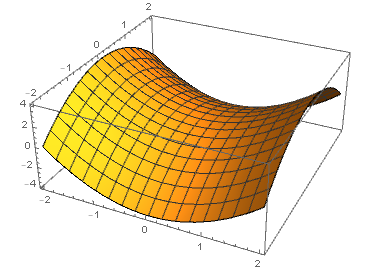
\includegraphics[scale=0.5]{images/rezsqr.png}
    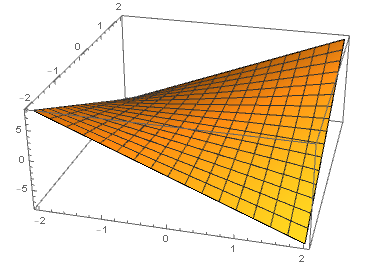
\includegraphics[scale=0.5]{images/imzsqr.png}
\end{center}
These graphs reveal a lot about how nice $u$ and $v$ are, but not a lot about the actual function $f$ itself. Sure, these will have their use/intuition when we investigate $u$ and $v$, but we need to be even more clever to get a nice visual representation of $f$.

Another idea is to instead graph the domain and range of $f$ separately -- that is, feed in a selected subset of $\CC$, and let Mathematica tell us where that maps to. That seems fairly reasonable! Below, we consider the image of the rectangle bounded by $1, 2, 1+3i, 2+3i$:
\begin{center}
    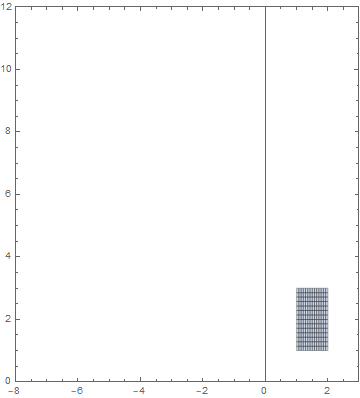
\includegraphics[scale=0.5]{images/domzsqr.png}
    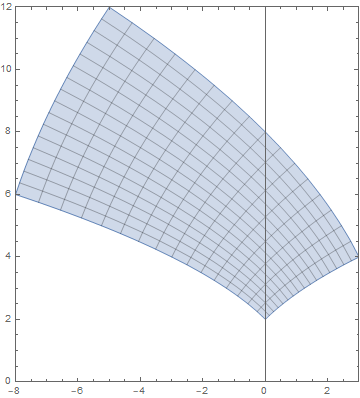
\includegraphics[scale=0.5]{images/ranzsqr.png}
\end{center}
Here, we see more geometrically what $z^2$ is doing -- it's doubling the arguments and rotating it, all the while the modulus is being squared and being pulled away from the origin. This captures the essence of the squaring function more completely than how our first method pulled the real and imaginary parts apart.

Notice also that I drew lines in my domain that represented lines of constant real/imaginary parts, and Mathematica graciously shows where these lines map to. While they don't remain straight, these curves still remain perpendicular to each other, which is a bit unexpected!

We go again, with the rectangle with vertices $-1+i, -1-i, 2+i, 2-i$:
\begin{center}
    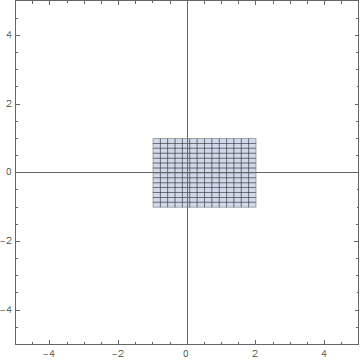
\includegraphics[scale=0.5]{images/domzsqr1.png}
    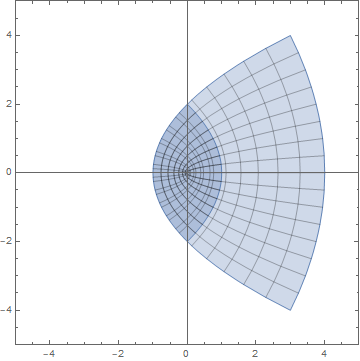
\includegraphics[scale=0.5]{images/ranzsqr1.png}
\end{center}
Let's see what happens if we were to walk around the image of the boundary of our domain in the output space. $2+i$ goes to $3+4i$, which corresponds to the top-right corner of the figure. We keep walking, keeping the interior to the left, until we reach the image of $-1+i = -2i$, past the other corner in the figure. We walk inside the figure, up to the other corner, and then overlap our own interior by walking to $3-4i$ and back up to the top-right. The orientation of the interior has still been preserved, and so has the angles between the lines, for the most part (except at 0). Functions which preserve angles and orientation in this manner are called \textit{conformal}. We'll discuss more conformal mappings in the following section.

Here's a mapping that's decidedly \textit{not} conformal -- $f(x + iy) = -y + xyi$:
\begin{center}
    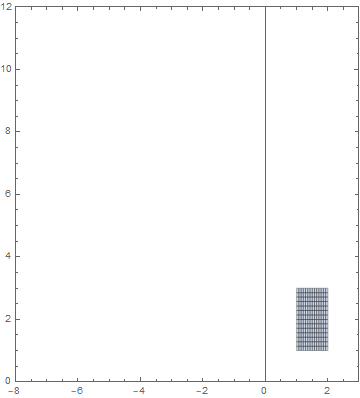
\includegraphics[scale=0.5]{images/domzsqr.png}
    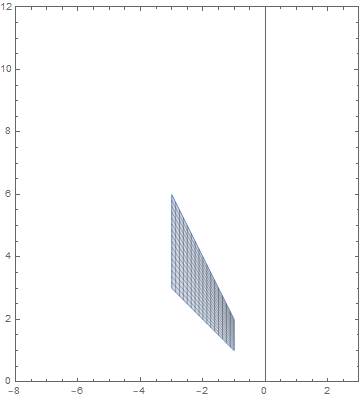
\includegraphics[scale=0.5]{images/ranzsqr2.png}
\end{center}
This, clearly, doesn't at all preserve angles by inspection, so not all functions $f(x+iy)$ with given $u(x, y)$ and $v(x,y)$ are conformal. We'll talk about what functions are and aren't conformal next time.

Finally, we turn to a fairly unorthodox, psychadelic method -- color maps. Normally, to establish a sort of baseline for ourselves, we first ``paint'' the entire complex plane with colors, varying hues for different arguments and making the saturation/brightness of the colors closer to the origin. We're not as concerned with the modulus, so we're just going to color the plane with the rainbow like so:
\begin{center}
    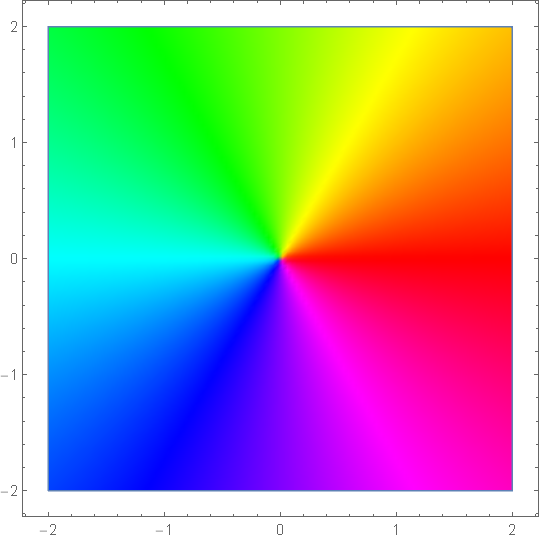
\includegraphics[scale=0.25]{images/colorbase.png}
\end{center}

For reference, the positive real axis is red, the positive imaginary axis is light green, the negative real axis is a light aqua, and the negative imaginary axis is purple.

To read these maps, the color of each point of the plane shows what argument the point maps to. Here's a color map of $f(z) = z^2$:
\begin{center}
    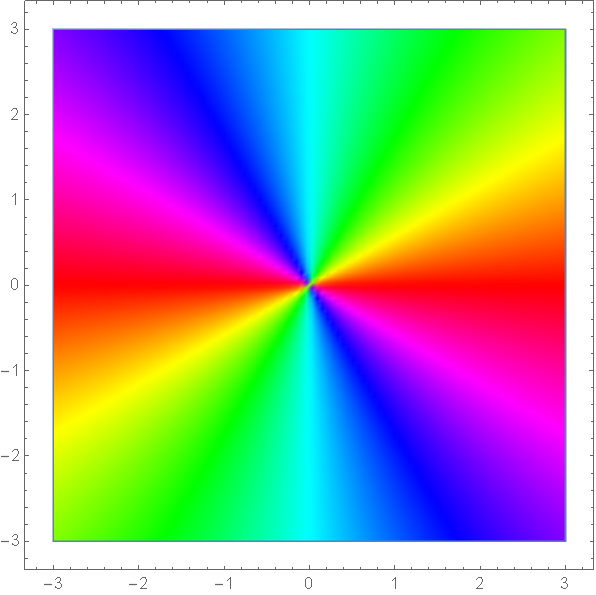
\includegraphics[scale=0.27]{images/colorzsqr.png}
\end{center}
Notice how the rainbow is repeated twice around the origin, as the we get to cycle through all of the different arguments twice. Here's $e^z$, and $\sin z$ for reference:
\begin{center}
    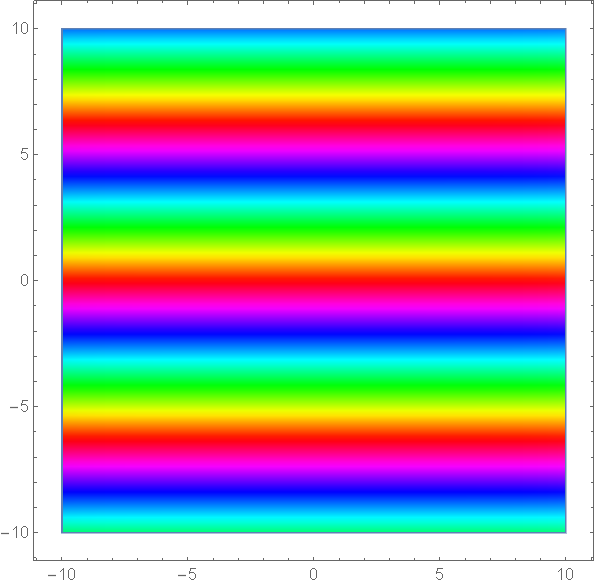
\includegraphics[scale=0.27]{images/colorez.png}
    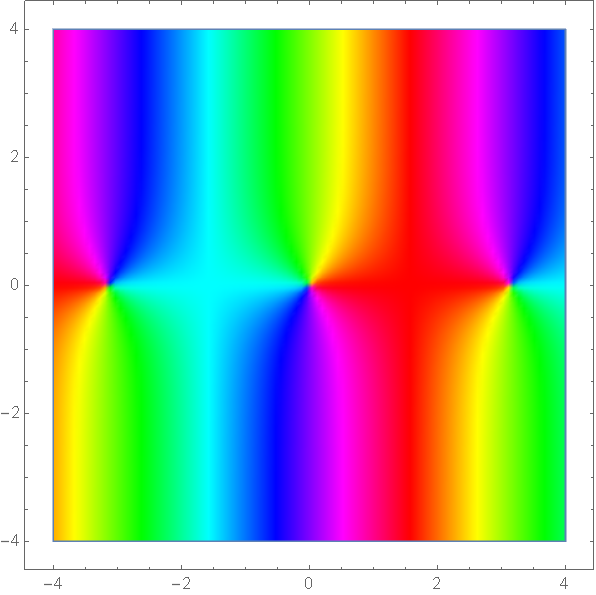
\includegraphics[scale=0.27]{images/colorsinz.png}
\end{center}
Note that the stripes on $e^z$ come from the periodicity every $2\pi$ in $e^ir$ for $r$ real, and we can see the regular periodicity in the $\sin$ function directly.

These color maps are going to be useful for visualizing discontinuities, which we will discuss later.
% conformality 

\section{Keeping Up With the M\"{o}biuseseses}
% riemann sphere and fractional linear transformations
M\"{o}bius transformations, or fractional linear transformations (FLTs), are worth studying as a sidenote here they are interesting conformal mappings of regions. These were discussed in HCSSiM's PJ 5, but I'll reiterate some of the main points here.

FLTs are functions of the form $f(z) = \frac{az+b}{cz+d}$, where $ad - bc \neq 0$ as to not make the function constant. They are compositions of translations ($f(z) : z \rightarrow z + c, c \in \CC$), rotations/dilations ($f(z) : z \rightarrow rz, r \in \CC$) and a reciprocation $\left(f(z) : z \rightarrow \frac{1}{z}\right)$. Because of this, they can established to be conformal by how they are constructed, geometrically (regular geometric inversion preserves angles, but not orientation... see if you can work this one out!).

In particular, FLTs are nice because they send circles and lines to circles and lines. This is true by construction for translations, rotations, and dilations, but reciprocations require breaking the function down into its real and imaginary parts and computing this explicitly.

Currently, the point $z = - \frac{d}{c}$ is a pole, unless we work in the \textit{one-point compactification of the complex plane}, which is just fancy math speak for ``adding $\infty$ to $\CC$ to complete the plane.'' This also allows us to have $\frac{a}{c}$ in our range, if we're allowed to plug in the point at infinity into our FLTs.

FLTs are fixed by three points -- we can always construct transformations that send the numbers $z_1$, $z_2$, and $z_3$ to $0, \infty$, and 1, respectively, like so:
\[
    f(z) = \frac{z_3-z_2}{z_3-z_1} \cdot \frac{z-z_1}{z-z_2}
\]
That means if we want to generally send $z_1 \rightarrow w_1$, $z_2 \rightarrow w_2$, and $z_3 \rightarrow w_3$, we can construct $f(z)$ such that $z_1 \rightarrow 0$, $z_2 \rightarrow \infty$, and $z_3 \rightarrow 1$, as well constructing $g(z)$ such that $w_1 \rightarrow 0$, $w_2 \rightarrow \infty$, and $w_3 \rightarrow 1$. Then, we can take $h(z) = g^{-1}(f(z))$ to get the unique transformation we want, which shows that transformations are fixed by three points.

With all of that summary out of the way, I'm most interested in talking about looking at the domain/range graphs when it comes to the FLTs. In all of the following examples, I'll provide the domain, and its output range. Note that all of these are conformal -- they preserve orientation and angles, even if they don't look like it! A good way to check orientation -- if you walk around the boundary counterclockwise (including through infinity), the interior should be to the left.

Okay, here are the pictures, and all of them are pretty wacky.  I tried to make Mathematica as unhappy as possible by using the reciprocation as much as possible, so these will look weird:
\begin{center}
    1. $f(z) = \frac{z-1}{z}$ on unit disk $|z| \leq 1$: \\
    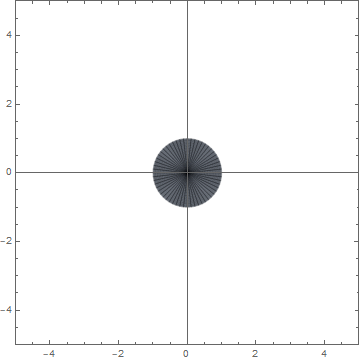
\includegraphics[scale=0.3]{images/mobius1dom.png}
    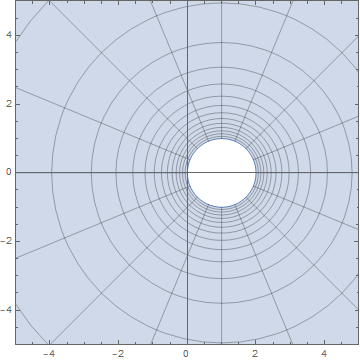
\includegraphics[scale=0.3]{images/mobius1ran.png}
\end{center}
\begin{center}
    2. $f(z) = \frac{z+1}{-z+1}$ on unit disk $|z| \leq 1$: \\
    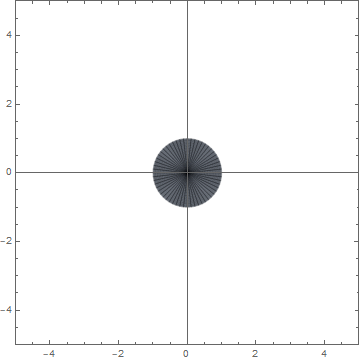
\includegraphics[scale=0.3]{images/mobius1dom.png}
    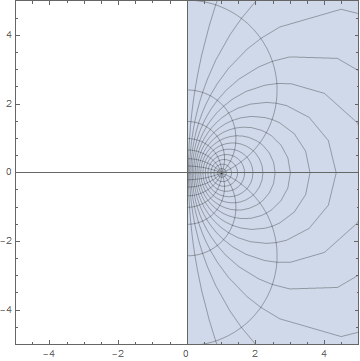
\includegraphics[scale=0.3]{images/mobius2ran.png}
\end{center}
\begin{center}
    3. $f(z) = \frac{1}{z}$ on square -- $\Re(z) \in [-1,1], \Im(z) \in [-1,1]$: \\
    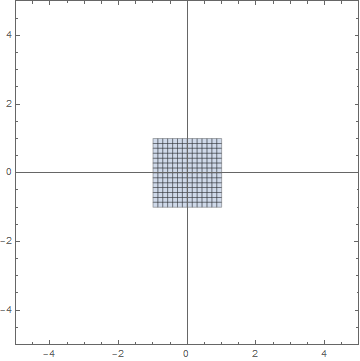
\includegraphics[scale=0.3]{images/mobius3dom.png}
    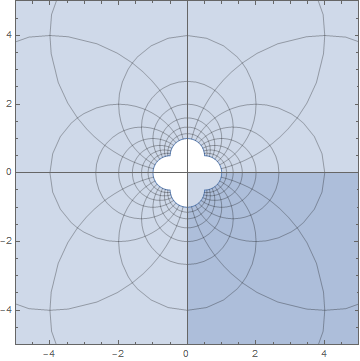
\includegraphics[scale=0.3]{images/mobius3ran.png}
\end{center}
\begin{center}
    4. $f(z) = (1+i)\frac{z-1}{z-i}$ on square -- $\Re(z) \in [0,1], \Im(z) \in [0,4]$: \\
    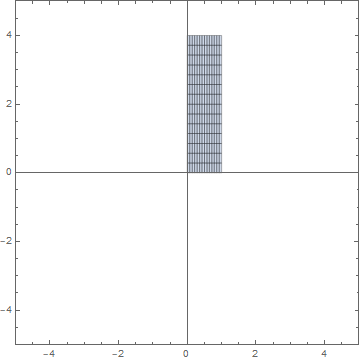
\includegraphics[scale=0.3]{images/mobius4dom.png}
    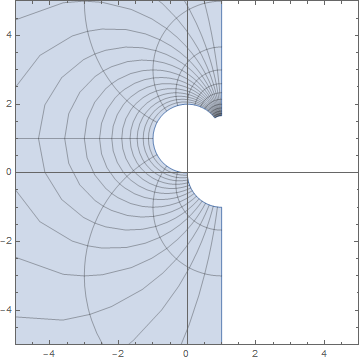
\includegraphics[scale=0.3]{images/mobius4ran.png}
\end{center}
The third example is an example of where Mathematica tries to connect the different infinities encountered near zero, and it ends up overlapping one of the quadrants. I'm not sure how to fix this, because the region is really only supposed to be the plane, minus the cloverleaf in the middle. Work it out for yourself to verify this! Try mapping each of these (directed) segments seperately, remembering to keep the interior to the left. :)
\section{Completing the Calculator}
% exp, sin, cos, sinh, cosh, tanh, Log, Arcsin, Arccos, Arctan

Recall the exponential function $e^z$, which we originally took as the function that satisfies the differential equation $y' = y$ and initial condition $y(0) = 1$. We can equivalently define it over all $\CC$ in terms of its Taylor series $e^z = 1 + z + \frac{z^2}{2!}  + \frac{z^3}{3!} + \cdots$, which is convergent everywhere, but we're not really concerned with the underpinnings of this function from a qualitative analysis for right now. What's more important to us right now is how many other functions the exponential function gives rise to, and why it's so important.

The first of these are $\sin$ and $\cos$ -- these are real functions that can be generalized using Euler's Formula to complex numbers:
\[
    \cos \theta = \frac{e^{i\theta} + e^{-i\theta}}{2} \quad \sin \theta = \frac{e^{i\theta} - e^{-i\theta}}{2i}
\]
These are consistent with the real-number definitions of $\sin$ and $\cos$, and extend this function to the entire complex plane. If we take, for example, $\sin(x+iy)$, for $x, y$ real, we get (after applying this definition)
\begin{align*}
    \sin (x+iy) & = \frac{e^{i(x+iy)}- e^{-i(x+iy)}}{2i} = \frac{e^{-y + ix}- e^{y - ix}}{2i}                     \\
                & = \frac{e^{-y}(\cos x + i \sin x) - e^{y}(\cos x - i \sin x)}{2i}                               \\
                & = \sin x \left(\frac{e^y + e^{-y}}{2} \right) + i \cos x \left(\frac{e^{y} - e^{-y}}{2} \right)
\end{align*}

This leads us to define very close relatives of the sine and cosine -- the \textit{hyperbolic sine and cosine}, denoted $\sinh$ and $\cosh$. We'll let
\[
    \sinh x = \frac{e^{x} - e^{-x}}{2} \quad \cosh x = \frac{e^x + e^{-x}}{2}
\]
Essentially, it's the same definition as sine and cosine with exponential functions, removing any $i$s that appear. This means that
\[
    \sin(x +iy) = \sin x \cosh y + i \cos x \sinh y
\]
If we were to compare this to a use of the sine addition formula:
\[
    \sin(x + iy) = \sin x \cos(iy) + \cos x \sin(iy)
\]
This allows us to conclude that
\[
    \cosh y = \cos (iy) \quad \sinh y = -i \sin(iy),
\]
by comparing terms. Of course, we could have deduced this relationship directly from the definitions as well.

The hyperbolic sine and cosine behave very similarly to our regular trig functions, but with some properties flipped around. For example, consider $\cosh^2 x$ and $\sinh^2 x$ when added and subtracted (these are the squares of $\cosh, \sinh$):
\[
    \cosh^2 x - \sinh^2 x = 1 \quad \cosh^2 x + \sinh^2 x = \cosh 2x
\]
If we define $\tanh x$, $\sech x$, $\csch x$, and $\coth x$ similarly to how their regular trigonometric counterparts are defined (i.e. $\frac{\sinh x}{\cosh x}, \frac{1}{\cosh x}, \frac{1}{\sinh x}, \text{ and } \frac{\cosh x}{\sinh x}$, we see that this yields the very similar
\[
    1 - \tanh^2 x = \sech^2 x \quad \coth^2 x - 1 = \csch^2 x.
\]
These are all analogues of the ordinary Pythagorean identities.  Recall the Pythagorean identity comes from a geometric interpretation of these functions -- if we let $\cos \theta$ correspond to $x$, and $\sin \theta$ correspond to $y$, we get a nice parameterization of a unit circle. Similarly, letting $x$ correspond to $\cosh t$ and $y$ correspond to $\sinh t$ gives $x^2 - y^2 = 1$, a hyperbola! This is the reason for calling these functions hyperbolic in nature.

The derivatives of these functions behave a bit more nicely than the regular trig functions:
\[
    \dv{}{z} \sinh z = \cosh z \quad \dv{}{z} \cosh z = \sinh z
\]
Note the absence of the minus sign on the derivative of $\cosh z$! It was present before because of the extra $i$ that $\sin$ and $\cos$ had, but no more. One can derive the other corresponding derivatives of $\tanh z, \coth z, \sech z, \csch z$. Interestingly, all of them look the same as their trig counter parts, but $\sech z$ gets an extra minus sign\ldots the price you pay, I suppose.

We can also talk about the inverses of these functions! Define $w = \log z$ as a number for which $e^w = z$. Notice I didn't say \textit{the} number -- there are an infinite number of them for every complex number! Even for reals, for this function we've extended to $\CC$, something like $\log 2$ doesn't have a single value:
\[
    \log 2 = \log (2 e^{2\pi i n}), n\in \ZZ \implies \log 2 \in \{\ln 2 + 2\pi i n, n \in ZZ\}
\]
(Here, I distinguish between the real-valued $\ln x : \RR \to \RR$ and the complex $\log z$ for the logarithm, which is a distinction I will continue to use for clarity.)

This is a problem, which once again stems from the fact that numbers have infinitely many possible arguments, and that multiplying numbers by $e^{2\pi n}$ doesn't change them. Again, to remedy this, we present the \textit{principal log} function, $\Log (z)$, which forces the number to be written with a principal argument before the logarithm is taken. Hence,
\[
    \Log 2 = \ln 2,
\]
and everything is right in the world once more. Similarly, $\Log r = \ln r$ for all positive real $r$. We can also see the $\Log$ of other complex numbers:
\[
    \Log (1 + i \sqrt{3}) = \ln 2 + i \frac{\pi}{3} \quad \Log(4  - 4i) = \ln 4 \sqrt{2} - i \frac{\pi}{4}
\]
In general, see how we can write the $\Log$ function explicitly in its real and imaginary parts:
\[
    \Log z = \ln |z| + i \Arg(z)
\]
As always, 0 is a problem point, as 0 doesn't have an Argument - it has infinitely many, even with the principal branch. This is an issue that even the $\Log$ cannot avoid, but we can only expect so much.

With this in mind, we can actually write down the inverse trigonometric functions explicitly in terms of the $\Log$ function. This is done by letting $w = \sin z$ (or other trig function), creating a quadratic in $e^{iz}$, and using the quadratic formula and picking the right branch based on consistency with the regular, real-number inverse trig functions. This gives us
\[
    \Arcsin z = -i \Log\left(iz + \sqrt{1-z^2}\right) \quad \Arccos z = -i \Log\left(z + \sqrt{z^2 -1}\right) \quad \Arctan z = \frac{i}{2} \Log\left( \frac{1+iz}{1-iz}\right),
\]
where everything is done principally. This allows us (finally!) to take the $\Arcsin$ of numbers outside the real interval $[-1, 1]$, and instead take it of any complex number we want! In particular, $\Arcsin 2$ exists -- it's just a complex number, which happens to be
\[
    \Arcsin 2 = -i \Log(2i + \sqrt{1-4}) = -i \Log\left(2+\sqrt{3}i\right)
\]
This, for the most part, addresses most of the functions on your handy-dandy scientific calculator that it has buttons for, in all of $\CC$ -- all stemming from the exponential function.
\section{Ripped to Pieces}
% b r a n c h c u t s 

Recall that in order to make the argument a function, we limited the range of the Argument such that $Arg(z) \in (-\pi, \pi]$. In a sense, we had taken a large cleaver and cut off the other infinitely many values for the argument of a number. At the places where $\Arg(z) = \pi$, then, we get an infinite discontinuity in the function all along the negative real axis, and at 0. This discontinuous ``cut'' in the function we call a \textit{branch cut}. Strange, strange things happen because of this choice, and we'll explore this now with the color maps.

Remember with the $\Log$ function, we wrote $\Log(z) = \ln|z| + i\Arg(z)$. Since the Argument function has a branch cut all along the negative real axis, we should also see a branch cut all along the negative real axis here -- and indeed, we do, looking at the color map of $\Log(z)$:
\begin{center}
    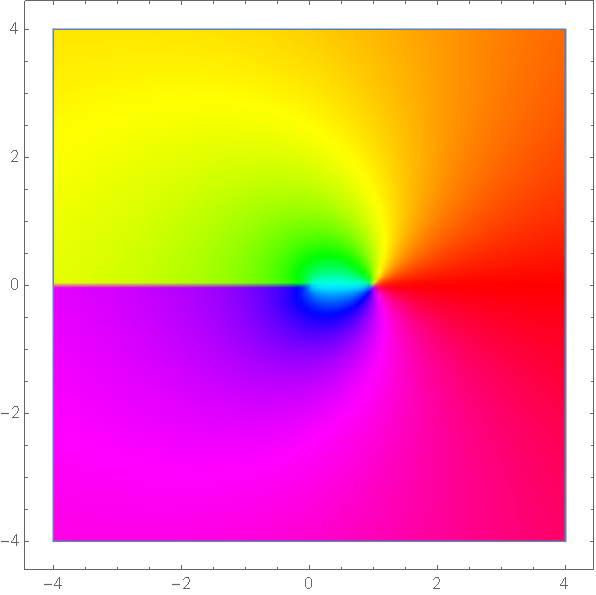
\includegraphics[scale=0.27]{images/colorlogz.png}
\end{center}
The branch cut here is displayed \textit{very} prominently in the sharp discontinuity in color crossing the negative real axis. Cuts can sometimes start and end at \textit{branch points}, and in this case, 0 is a branch point of $\Log(z)$. One subtlety to note is that a branch point must be present in every branch of the multi-valued function -- so some points that look like branch points might actually be illusory, which can be very confusing. In general, a good way to identify possible branch points is to ask where one is taking a $\Log$ or a non-integer power of 0 or $\infty$, and \textit{cuts always occur when one is taking a $\Log$ or non-integer powers of negative reals}.

We can use the color maps to look at the cuts in functions that look similar, but actually exhibit very different behaviors. For example, consider $\sqrt{z^2-1}$ and $z \sqrt{1-\frac{1}{z^2}}$:
\begin{center}
    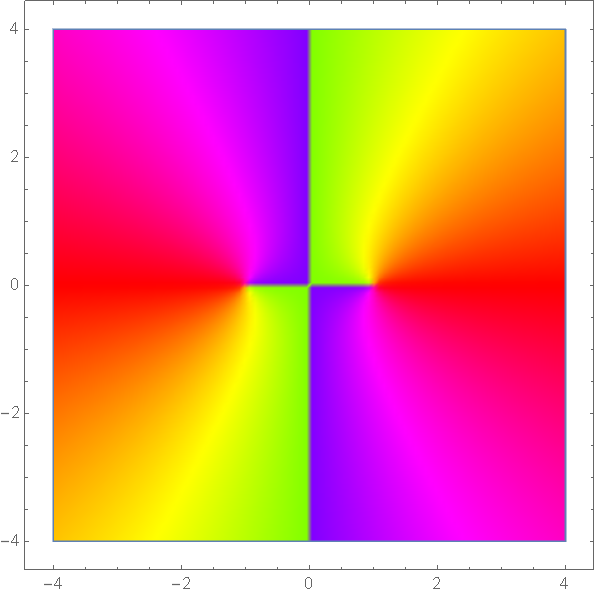
\includegraphics[scale=0.27]{images/sqrtzsqrminus1.png}
    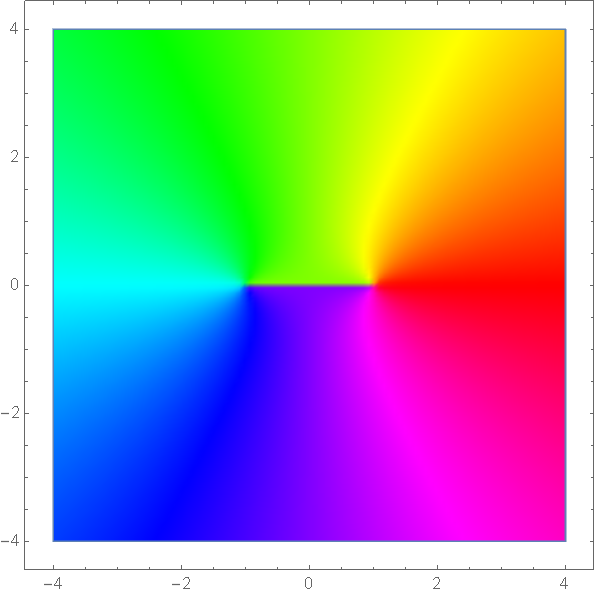
\includegraphics[scale=0.27]{images/sqrtzsqrminus2.png}
\end{center}
Here, both functions have branch points at $\pm 1$, but the first appears to have a branch cut running through infinity along the imaginary axis. However, we've just identified a branch of the function $(z^2-1)^{\frac{1}{2}}$ where $\infty$ doesn't appear along any cuts, so it's actually an illusory branch point.

Contrast this with $\sqrt[3]{z^2-1}$ and $z^{\frac{2}{3}} \sqrt[3]{1-\frac{1}{z^2}}$:
\begin{center}
    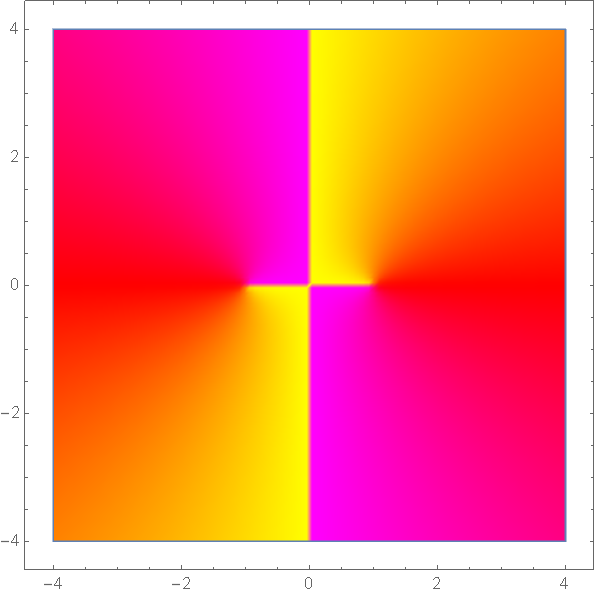
\includegraphics[scale=0.27]{images/cbrtzsqrminus1.png}
    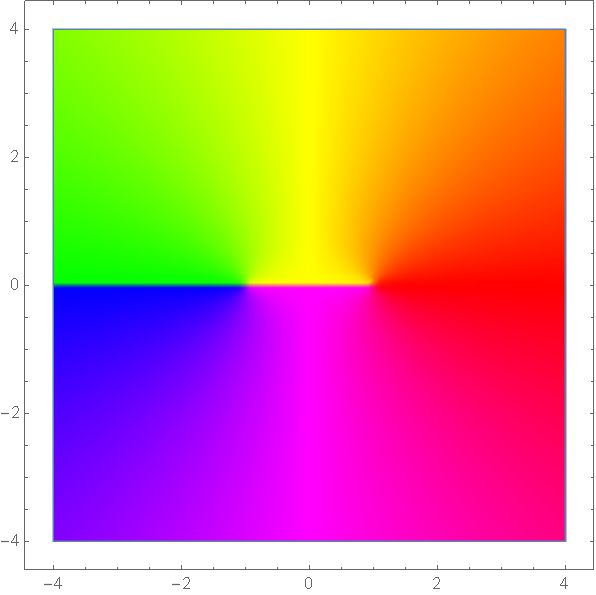
\includegraphics[scale=0.27]{images/cbrtzsqrminus2.png}
\end{center}
Notice that here, $\infty$ is an actual branch point! Taking out the $z^{\frac{2}{3}}$\footnote{Normally, this would be multi-valued, but I mean the principal branch of this function here. } out of the cube root doesn't actually remove the point at infinity, as this function inherently has a branch cut along the negative real line. $0$, however, is not a branch point of this function, as the first branch presented did not have it as a possible branch point. This manipulation has only made us move the cut through infinity in a strange manner.

On that note, we can see that functions that really should be the same, such as $(\sqrt{z})^2$ and $\sqrt{z^2}$, have different branch cuts, meaning that they're different branches of $z$. Here they are, respectively:
\begin{center}
    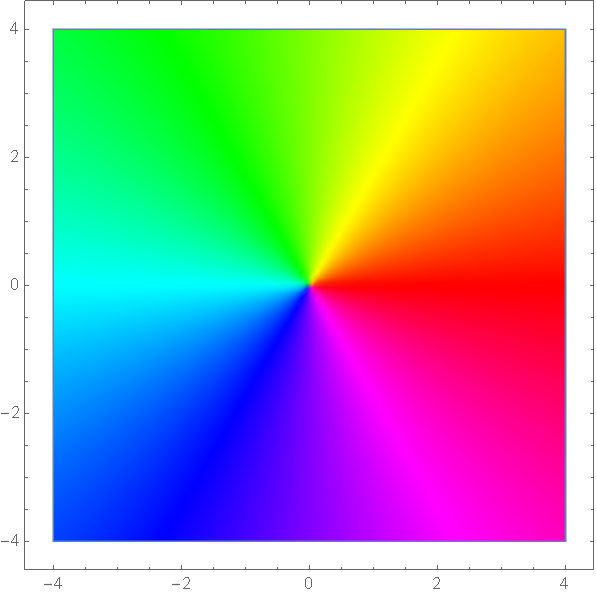
\includegraphics[scale=0.27]{images/sqrtzsqr1.png}
    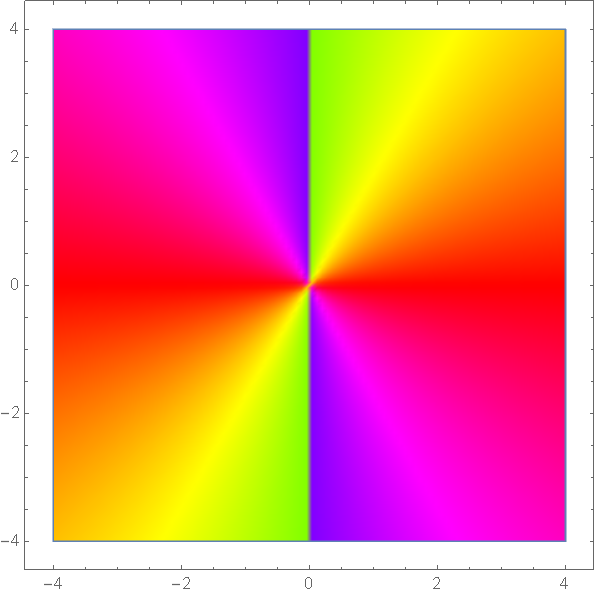
\includegraphics[scale=0.27]{images/sqrtzsqr2.png}
\end{center}
Notice the first function has no branch cuts anywhere -- we call these kinds of functions \textit{entire}, although that's not the proper definition of the term.

Similarly, $\sqrt[3]{z^2}$ and the principal branch of $z^{\frac{2}{3}}$ are different branches of the same function as well, evidenced by their branch cuts, and we show them here, respectively:
\begin{center}
    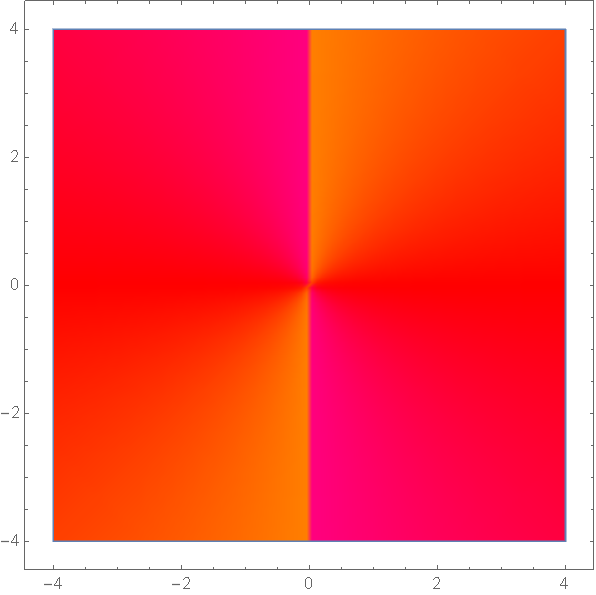
\includegraphics[scale=0.27]{images/cbrtzsqr1.png}
    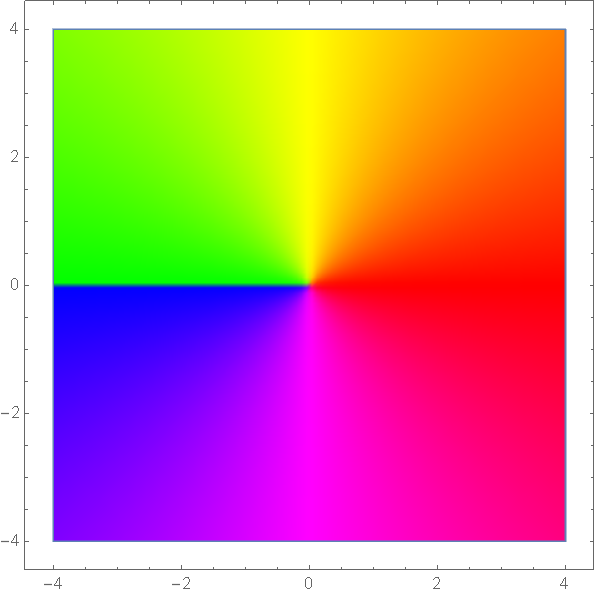
\includegraphics[scale=0.27]{images/cbrtzsqr2.png}
\end{center}
This is all very, very strange! This choice that we made in Section 1 has rent asunder what we think should be obviously true about these functions. Moving forward, whenever we see a function that has some sort of non-integer power, or has a Log, we should be careful to see where the branch cuts \textit{actually} are, because they can be very, very tricky.

For your viewing pleasure, I present a few more pretty color plots -- see if you can figure out for yourself why the branch cuts are in the places you see them! Feel free to come up with different branches of the multi-valued functions, if you can, that will eliminate illusory branch points as well. If a function looks multi-valued, assume I'm always using the principal branch.

\begin{center}
    1. $f(z) = \sqrt[3]{z^6-1}$ \\
    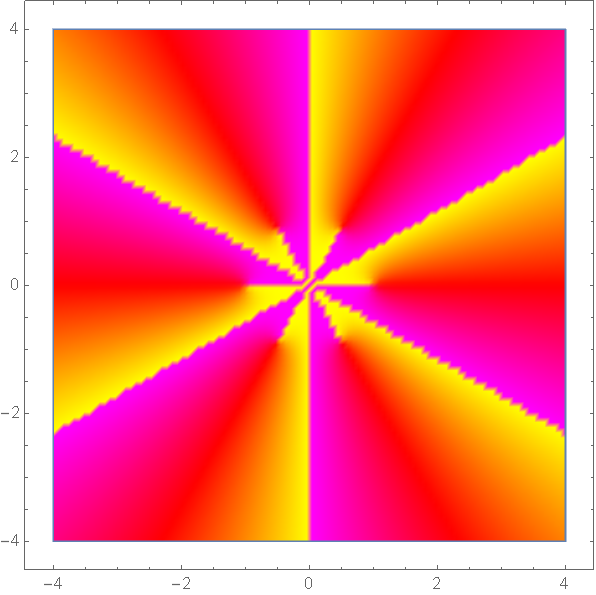
\includegraphics[scale=0.27]{images/cbrtzsixminus1.png}
\end{center}
\begin{center}
    2. $f(z) = \sqrt{z^4-1}$ vs. $f(z) = i\sqrt{1-z^4}$ \\
    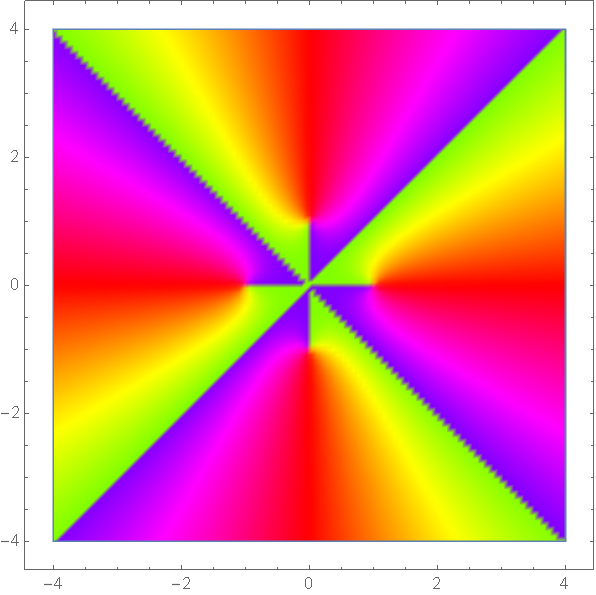
\includegraphics[scale=0.27]{images/poszfourminus1.png}
    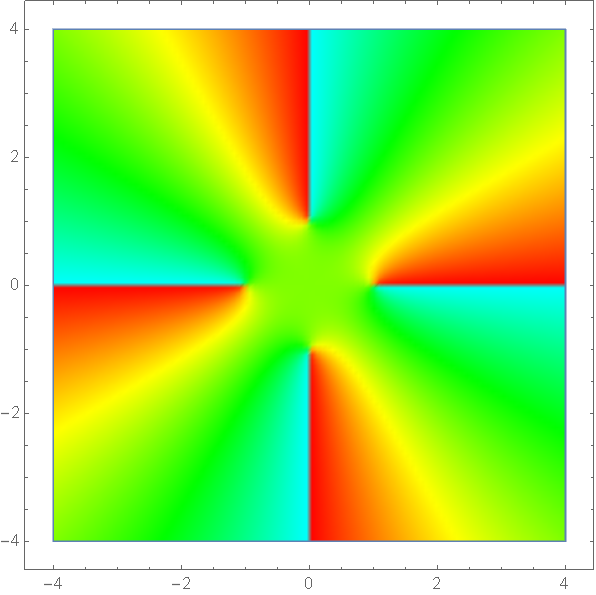
\includegraphics[scale=0.27]{images/negzfourminus1.png}
\end{center}
\begin{center}
    3. $f(z) = \left(\frac{1-z^2}{1+z^2}\right)^i$: \footnote{This one has branch cuts due to the modulus, and not the argument, so I've added back the saturation/brightness functions to show this effect. Darker means closer to 0, brighter means closer to infinity.}\\
    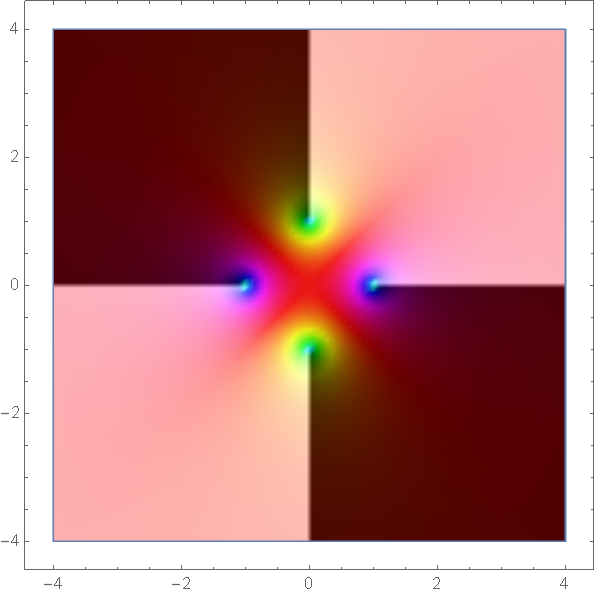
\includegraphics[scale=0.27]{images/weirdpower.png}
\end{center}
Feel free to mess around with any other weird functions with branches on your own!

\pagebreak

\section{The Best Functions}

We begin our foray into complex analysis and start with a discussion of the smooth functions on $\CC$. We'll soon see that these are actually incredibly nice!

\subsection{Topology of the Complex Numbers}
Before we start talking about analysis in $\CC$, we should establish what the topology on $\CC$ is. It's not at all unfamiliar -- it's essentially just like $\RR^2$! Remember that the norm $\norm \cdot$ on $\CC$ that we looked at in the last section gives $\CC$ a metric space structure that looks almost exactly like the absolute value between points in $\RR^2$. Recall:
\begin{definition}
  A \textbf{metric space} is a space $X$ with a \textbf{distance function} $d: X \times X \to \RR$ such that the following three statements are true:
  \begin{itemize}
    \item For all $x, y \in X$, $d(x,y) \geq 0$ and $d(x,y) = 0 \Leftrightarrow x = y$.
    \item For all $x, y \in X$, $d(x,y) = d(y,x)$.
    \item For all $x, y, z \in X$, $d(x,y) + d(y,z) \geq d(x,z)$.
  \end{itemize}
\end{definition}
Most of the analysis you have done so far has been in a metric space -- all your work in $\RR^n$ has been like this, and $\CC$ is no different.

The following definitions should look familiar -- again, it's literally just like $\RR^2$!
\begin{definition}
  An \textbf{open disk} of radius $r$ around $z_0$ in $\CC$ is the set of points $D_r(z_0) = \braces{z \in \CC : |z - z_0| < r}$.
\end{definition}
\begin{definition}
  A set $U \subseteq \CC$ is \textbf{open} if for every $z \in U$, there exists some $r > 0$ in $\RR$ such that $D_r(z_0) \subseteq U$.
\end{definition}
(Note that the ``in $\RR$'' is a little redundant, as $\CC$ cannot be totally ordered -- so if a total ordering is implied, we have should be assumed to be in $\RR$.)
\begin{definition}
  A set $V \subseteq \CC$ is \textbf{closed} if its complement $\CC - V$ is open.
\end{definition}

We also establish limits of sequences in pretty much the same way:
\begin{definition}
  A sequence of complex numbers $\braces{z_i}_{i=1}^\infty$ \textbf{converges} to some $w \in \CC$ iff \[ \forall \eps > 0, \exists \, n \in \NN : \forall n > N, |z_n - w| < \eps. \] If this is true, then we write $\lim_{n \to \infty} z_n = w$.
\end{definition}
It should be said that addition and multiplication of limits of sequences works exactly the same as in $\RR^n$.

\begin{definition}
  A point $w$ is a \textbf{limit point} of some set $U \subseteq \CC$ if there exists some sequence $\braces{z_n}$ in $U$ such that $\lim_{n \to \infty} z_n = w$.
\end{definition}

\begin{definition}
  The \textbf{closure} of a set $U$ in $\CC$, $\ol U$, is the union of $U$ with all its limit points.

  (As the name indicates, the closure of a set is closed -- this follows the same proof from Hubbard, more or less.)
\end{definition}

\begin{definition}
  The \textbf{interior} of a set $U$, $\inter U$, is the set of all points $z \in U$ such that there exists some $D_r(z) \subseteq U$.
\end{definition}

\begin{definition}
  The \textbf{boundary} of a set $U$ is $\closu U - \inter U$.
\end{definition}

Compactness topologically usually means dealing with open covers, but in a metric space, closedness and boundedness is enough:
\begin{definition}
  A set $U$ is \textbf{compact} if any cover of $U$ by open sets $\braces{U_\alpha}$ such that $U \subseteq \bigcup_\alpha U_\alpha$ has a finite subset of some $U_{\alpha_i}$ for $1 \leq i \leq n$ for some finite $n$ such that $U \subseteq \bigcup_{i=1}^n U_{\alpha_i}$. In other words, any open cover of $U$ has a finite subcover.

  Equivalently, a compact set $U$ in $\CC$ is closed and bounded, just as in Hubbard. (These happen to be equivalent because we're in a metric space!)
\end{definition}

Finally, we should recall that $\CC$ is \textbf{complete}, just as $\RR$ is. This means that for any \textbf{Cauchy sequence} $\braces{z_n} \in \CC$ (meaning that for any $\eps > 0$, there exists $N \in \NN$ such that for any $m, n > N$, $|z_m - z_n| < \eps$) converges to some $z \in \CC$.

Note that completeness is equivalent to the \textbf{nested compact set property}, which states that if we have a sequence of nested compact sets $U_1 \supseteq U_2 \supseteq \dots \supseteq U_n \subseteq \dots$, such that the diameters of these sets $\textrm{diam}(U_n) = \sup_{z, w \in U_n} |z - w|$ are a sequence converging to 0, then the intersection of all of these $U_i$ is non-empty.
%% proof: https://math.stackexchange.com/questions/2386270/is-the-nested-set-property-equivalent-to-cauchy-completeness ?? but also in the book

We will have a lot to say about \textbf{connectedness} as well. A set $U \subseteq \CC$ is connected if for any two $z, w \in U$ that there is a \textbf{path} joining $z$ and $w$ in $U$. In particular, this means there exists a continuous map $\gamma: [0,1] \to U$ such that $\gamma(0) = z$ and $\gamma(1) = w$. We will be very interested in paths, especially when we study integration.\footnote{This is actually not the proper definition of ``connected'' -- I've just given you the definition for ``path-connected''ness instead, which is a little stronger but are equivalent in $\CC$.}

A special variety of a connected set is a \textbf{simply connected} set. A simply connected set can be thought of as a set that ``has no holes in the middle'', so that it's sort of convex. Rigorously, we'll say that $U$ is simply connected if it and its complement, $\CC - U$ are both connected.\footnote{Again, this actually isn't the full definition -- the real definition requires a little bit of homotopy. Basically, we want all loops in the set to be contractible to a point, so that loops are homotopy-equivalent to a constant map. This means that you can continuously deform a loop and squish it down into a point. This is a pretty important notion in algebraic topology, but as a loose concept it will be really important here for us in complex analysis.}
%% connectedness

%% simple connectedness

Okay, that's enough topology. Hopefully most of this is review from 2230!

\subsection{Limits and Continuity}
We now turn to a discussion of limits and continuity of functions in $\CC$, but again, it's literally just like $\RR^2$! But for completeness, we rehash the definitions here.

\begin{definition}
  Let $U \subseteq \CC$. A function $f : U \to \CC$ has a \textbf{limit} $w$ at $z_0$ if for all $\eps > 0$ there exists some $\delta > 0$ such that for all $z \in U$, \[ 0 < | z - z_0 | < \delta \Rightarrow |f(z) - w| < \eps .\] We say then that $\lim_{z \to z_0} f(z) = w$.
\end{definition}
\begin{definition}
  If $U \subseteq \CC$, and $f : U \to \CC$, then $f$ is \textbf{continuous} at $z_0$ if $f(z_0) = \lim_{z \to z_0} f(z)$.
\end{definition}
A slight note here -- Hubbard's definition of a limit is slightly different/non-standard. Hubbard's condition is instead that $ | z - z_0 | < \delta \Rightarrow |f(z) - w| < \eps$, which essentially forces a limit to exist for $f$ at a point $z_0$ if and only if the function $f$ is just continuous at $z_0$. It's kinda nice, but it's a little strange, I guess.

Of course, sequential continuity is equivalent to continuity -- if we have a sequence $\braces{z_n}$ converging to $z$ in $\CC$, and $f : U \to \CC$ where $U$ is some subset of $\CC$, $\lim_{n \to \infty} f(z_n) = f(z)$. Also, all the standard limit/continuity theorems for combining functions apply. Addition/multiplication/composition of limits behave as expected, and same with continuity.


\subsection{Holomorphicity}
We move to the notion of differentiability on $\CC$. Differentiability

\begin{definition}
  Let $U$ be an open subset of $\CC$. A function $f : U \to \CC$ is \textbf{holomorphic} at $z_0 \in U$ if the limit $\lim_{z \to z_0} \frac{f(z) - f(z_0)}{z - z_0}$ exists. If it exists, the limit is denoted $f'(z_0)$, and is called the \textbf{derivative} of $f$ at $z_0$.

  If this holds at every point $z_0 \in U$, then $f$ is said to be holomorphic on $U$.
\end{definition}


Naturally, this definition of the derivative follows the same rules as the real derivative -- it's linear, and follows the product rule and chain rules, with the proofs being roughly the same as in $\RR^2$.

Here's where it starts to get weird. Let's investigate $f$ as a transformation from ``$\RR^2$'' to ``$\RR^2$''. In particular, if we think $f(x + iy) = u(x,y) + i v(x,y)$, then we have the following theorem about the real/imaginary parts of the function related to the real/imaginary parts of the input:
\begin{theorem}[Cauchy-Riemann]
  If $U \subseteq \CC$ is open, then $f : U \to \CC$ is holomorphic on $U$ iff \[ \pdv u x = \pdv v y \quad \pdv u y = - \pdv v x\] everywhere in $U$.
  These equations are called the \textbf{Cauchy-Riemann equations} and can be used as a criterion for holomorphicity.
\end{theorem}

proof needed here
%% Cauchy 

\subsection{Power Series}
One thing we will do extensively later on is talk about power series. Here, I'll briefly talk about power series and convergence and analyticity.

\pagebreak


\end{document}